%******************************************************************************************************
%*********************************** First Chapter ****************************************************
%******************************************************************************************************

\chapter{Introduction}  %Title of the First Chapter
\label{intro}

% **************************** Define Graphics Path **************************
\ifpdf
    \graphicspath{{Chapter1/Figs/Raster/}{Chapter1/Figs/PDF/}{Chapter1/Figs/}}
\else
    \graphicspath{{Chapter1/Figs/Vector/}{Chapter1/Figs/}}
\fi


%******************************************************************************************************
%******************************************************************************************************
\section{An Introduction to Unmanned Aerial Vehicles} 
\label{intro:UAVs}

The term Unmanned Aerial Vehicle (UAV) can be used to describe any form of aircraft that does not require a pilot on board. This term includes aircraft that are controlled remotely, autonomous vehicles capable of navigating themselves, and any aircraft that are a combination of the two. Other terms that may be familiar are ``drone'' and Unmanned Aerial System (UAS), which can be used interchangeably with UAV within the context of this project. 

UAVs come in a wide range of form factors but can be split into two main classes; fixed-wing UAVs and rotary wing UAVs. Fixed-wing UAVs are generally only capable of horizontal take-off and landing (HTOL), whilst rotary wing UAVs generally employ vertical take-off and landing (VTOL). There are, however, other forms of UAV which incorporate features of both main classes; for example, quadplane UAVS use rotary wing rotors to allow VTOL, but do the main bulk of their flying with forward facing rotors much like a fixed-wing UAV. Across these categories are a very wide range of UAV platforms, from hobbyist quadcopters to military attack vehicles, and many many others in between. %TODO images?  
Although the range of UAV form factors and their uses is vast, the vast majority are suitable for candidates for complete autonomous flight control, as shall be described in Section %TODO reference where we talk about adding hardware modules 
 
Although there were a large number of suitable candidates for the following work, it was decided that this project would be aimed at the control of strictly fixed-wing UAVs for the purposes of aerial photography. For that reason, we shall not discuss any other style of UAV. %TODO 

%******************************************************************************************************
%******************************************************************************************************
\section{UAVs for Aerial Photography} 
\label{intro:photography}

The first recorded use of aerial photography was in 1858 by a French balloonist and photographer known as ``Nadar'' at a height of 80 metres using a tethered hot air balloon. %TODO ref aerial photography history
Since then aerial photography has of course massively progressed, both in terms of the aerial vehicles in use and the cameras available. As such, it is now an activity that can be partaken in by both organisations, companies, and individuals alike, for a range of purposes. For example, aerial photography of course plays a very large role in intelligence gathering by government agencies and militaries, but can also be a hobby for otherwise earth-bound photography enthusiasts. 

Different applications will require different equipment and styles of photography; a hobbyist may want a wide panorama, whilst a mapping application will require a consistent vertical camera angle. The use of aerial photography for mapping or measurement is known as aerial photogrammetry, and will be the chosen field of interest for this project. Aerial photogrammetry is a specific subset of aerial photography in that it not only requires the capturing of images, but additional information about how and where the image was captured. For this project, we are looking at the use of aerial photogrammetry to create an image of the land below our UAV. In order to be able to do this, we need to be able to capture a set of images, and know the location of the UAV when the images were captured, to allow the images to be stitched together into one larger image of the ground beneath. In this scenario we can typically use GPS co-ordinates and a pre-planned imaging path to define which images relate to which areas of the ground below. %TODO more






\begin{figure}[htbp!] 
\centering    
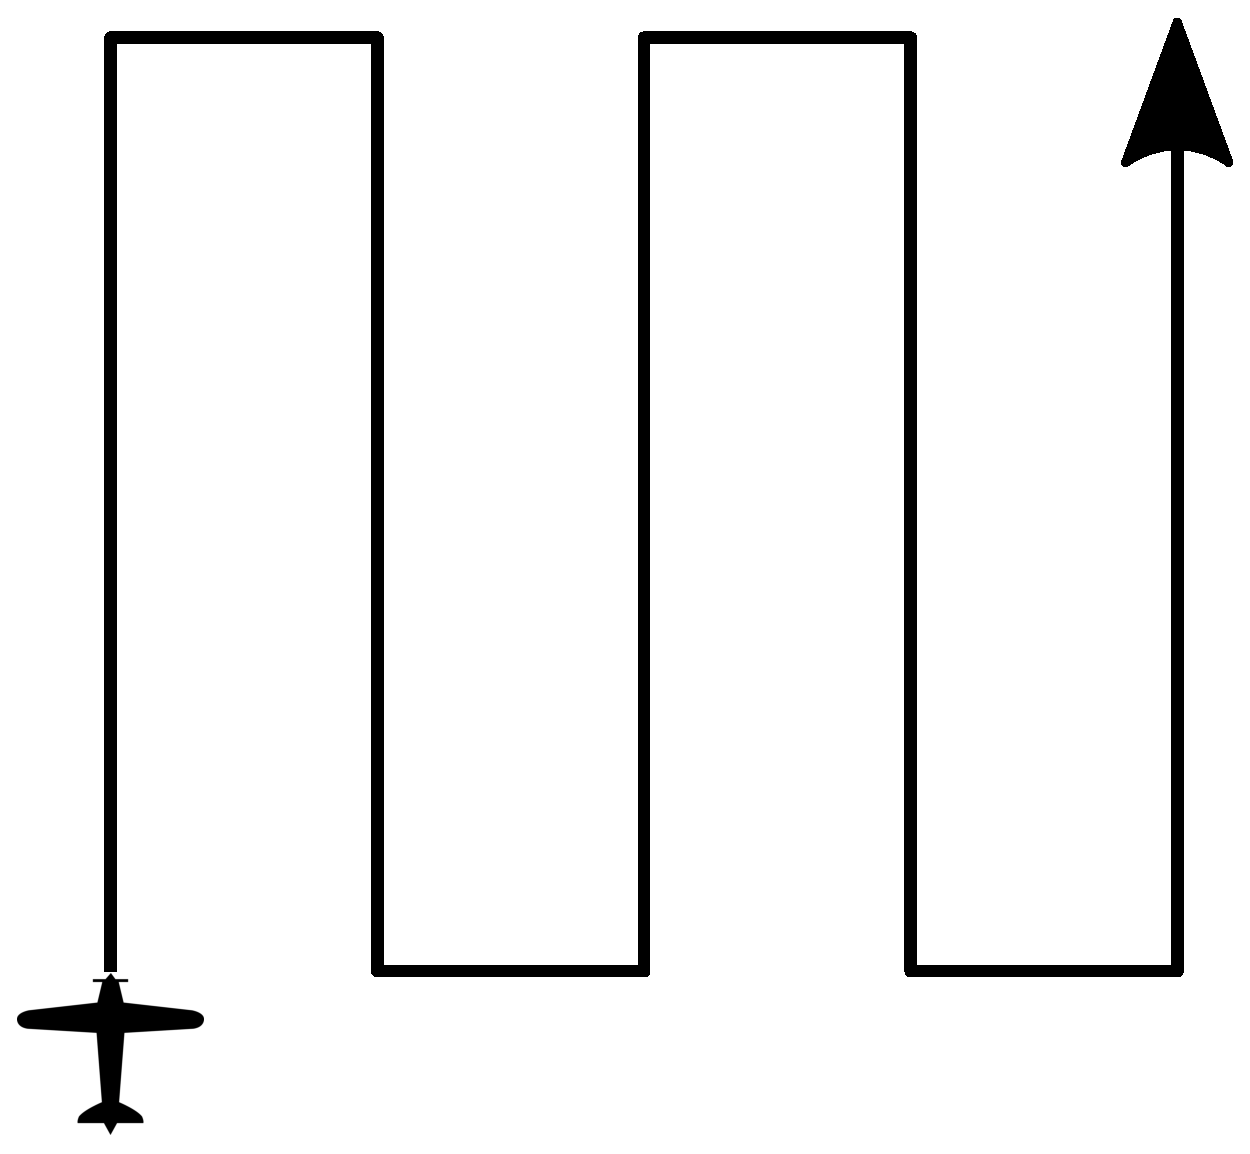
\includegraphics[width=1.0\textwidth]{SimpleLawnmower}
\caption[Simple Lawnmower]{This is the general form of a lawnmower pattern aerial imaging run} %TODO
\label{fig:simplelawnmower}
\end{figure}


%******************************************************************************************************
%******************************************************************************************************
\section{ArduPilot and ArduPlane} 
\label{intro:arduplane}

ArduPilot is an open-source suite of autopilot products aimed at hobbyists and professionals alike 

\subsection{JSBSim}
\label{intro:jsbsim}

JSBSim is the simulator packaged with ArduPlane for testing purposes

%******************************************************************************************************
%******************************************************************************************************
\section{Autopilot Hardware} 
\label{intro:hardware}



